% (The MIT License)
%
% Copyright (c) 2023-2024 Yegor Bugayenko
%
% Permission is hereby granted, free of charge, to any person obtaining a copy
% of this software and associated documentation files (the 'Software'), to deal
% in the Software without restriction, including without limitation the rights
% to use, copy, modify, merge, publish, distribute, sublicense, and/or sell
% copies of the Software, and to permit persons to whom the Software is
% furnished to do so, subject to the following conditions:
%
% The above copyright notice and this permission notice shall be included in all
% copies or substantial portions of the Software.
%
% THE SOFTWARE IS PROVIDED 'AS IS', WITHOUT WARRANTY OF ANY KIND, EXPRESS OR
% IMPLIED, INCLUDING BUT NOT LIMITED TO THE WARRANTIES OF MERCHANTABILITY,
% FITNESS FOR A PARTICULAR PURPOSE AND NONINFRINGEMENT. IN NO EVENT SHALL THE
% AUTHORS OR COPYRIGHT HOLDERS BE LIABLE FOR ANY CLAIM, DAMAGES OR OTHER
% LIABILITY, WHETHER IN AN ACTION OF CONTRACT, TORT OR OTHERWISE, ARISING FROM,
% OUT OF OR IN CONNECTION WITH THE SOFTWARE OR THE USE OR OTHER DEALINGS IN THE
% SOFTWARE.

\documentclass{article}
\usepackage{../sqm}
\newcommand*\thetitle{Function Points}
\begin{document}

\plush{\sqmTitlePage{17}{}}

\qte
  {capers-jones.jpg}
  {From the start of the software era in the 1950s until roughly 1970, software cost estimating was performed \ul{manually}, using simple \ul{rules of thumb} or local estimating algorithms developed through trial and error methods.}
  {jones2007}

\qte
  {fred-brooks.jpg}
  {Our techniques of estimating are \ul{poorly developed}. More seriously, they reflect an unvoiced assumption which is quite untrue, i.e., that \ul{all will go well}.}
  {brooks1995mythical}

\qte
  {lawrence-putnam.jpg}
  {In general, the \ul{size} of the product in source \ul{statements} is \(S = C \times K^{1/3} \times t^{4/3}\), where \(C\) is a productivity constant, \(K\) is development effort, and \(t\) is time.}
  {putnam1978general}

\qte
  {barry-boehm.jpg}
  {We compute the \ul{estimated development effort} as the nominal development effort times the product of the effort multipliers for the 15 \ul{cost driver attributes}... A nominal development effort is estimated as a function of the product's size in delivered source \ul{instructions} in thousands (KDSI) and the project's development mode.}
  {boehm1984software}

\qte
  {cocomo-2.jpg}
  {Success in all types of organization depends increasingly on the development of customized software solutions, yet more than half of software projects now in the works will \ul{exceed} both their \ul{schedules} and their \ul{budgets} by more than 50\%.}
  {boehm2000}

Parametric Review of Information for Costing and Evaluation – Software (PRICE-S)

Software Evaluation and Estimation of Resources – Software Estimating Model (SEER-SEM).

Doty Model

\qte
  {allan-albrecht.jpg}
  {The general approach is to count the number of external user \ul{inputs}, \ul{inquiries}, \ul{outputs}, and master \ul{files} delivered by the development project. These factors are outward manifestations of any application. They cover all the functions in an application.}
  {albrecht1979measuring}

\pitch{\begin{multicols}{2}
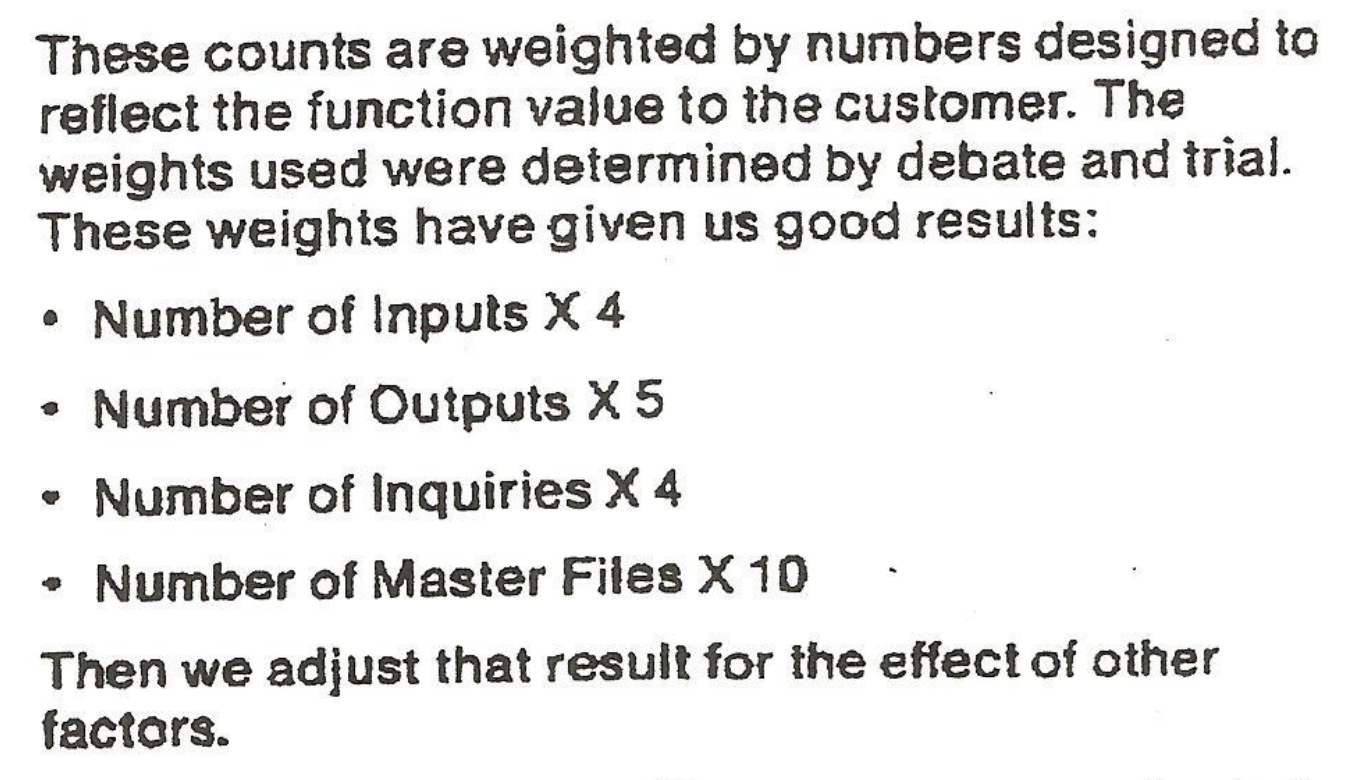
\includegraphics[width=\linewidth]{factors.png}
\par\columnbreak\par
``If the inputs, outputs, or files are extra complicated, we add 5\%. Complex internal processing can add another 5\%. On-line functions and performance are addressed in other questions. The maximum adjustment possible is 50\%, expressed as \(\pm\)25\% so that the weighted summation is the average complexity.''\par
{\scriptsize Source: \bibentry{albrecht1979measuring}\par}
\end{multicols}}

\qte
  {sloc-vs-fps.png}
  {At least for the applications analyzed, both the development work-hours and application size in ``SLOC'' are \ul{strong functions} of ``function points'' and ``input/output data item count.'' Further, it appears that basing applications development effort estimates on the amount of function to be provided by an application rather than an estimate of ``SLOC'' may be \ul{superior}.}
  {albrecht1983software}

\qte
  {capers-jones.jpg}
  {The reliability of function point analysis is good enough to allow function points to serve as the \ul{basis} for contracts, for carrying out scholarly research, for cost estimating, and for creating reliable benchmarks. In fact, function points are now \ul{used} for more business purposes than any other metric in the history of software.}
  {iso20926foreword}

\plush{
\pptBanner{IFPUG Procedure}
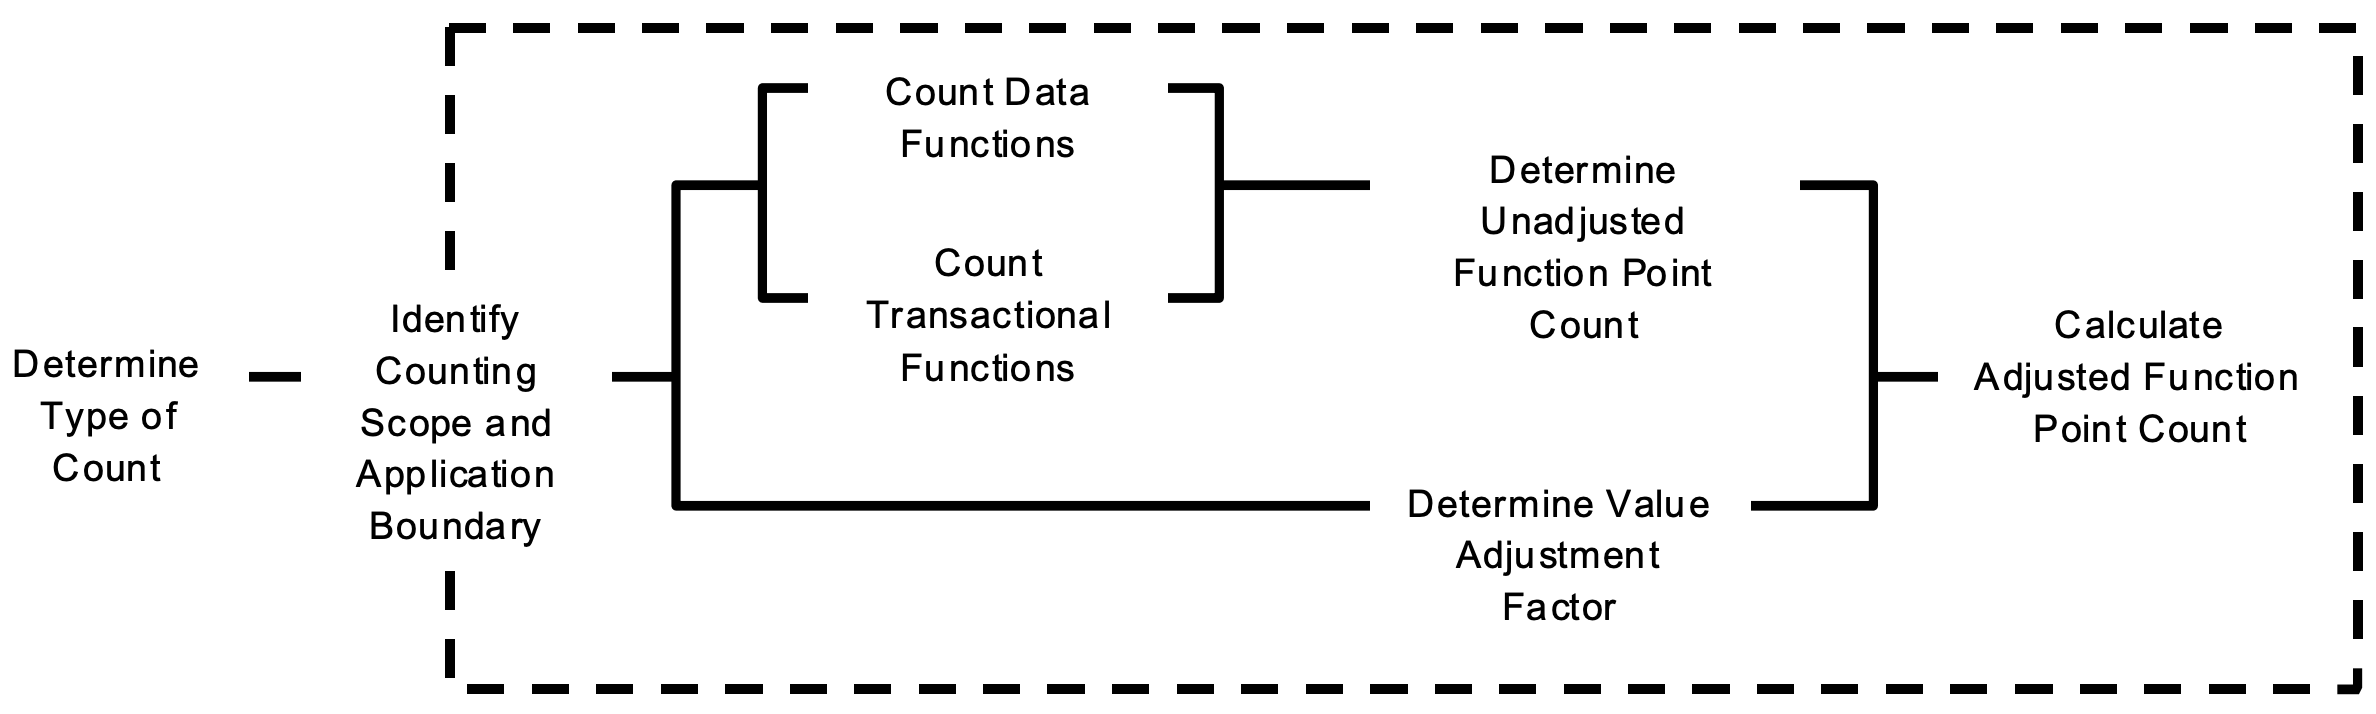
\includegraphics[width=\linewidth]{ifpug-procedure.png}
\par
{\scriptsize Source: \bibentry{iso20926}\par}}

\pitch{\begin{multicols}{2}
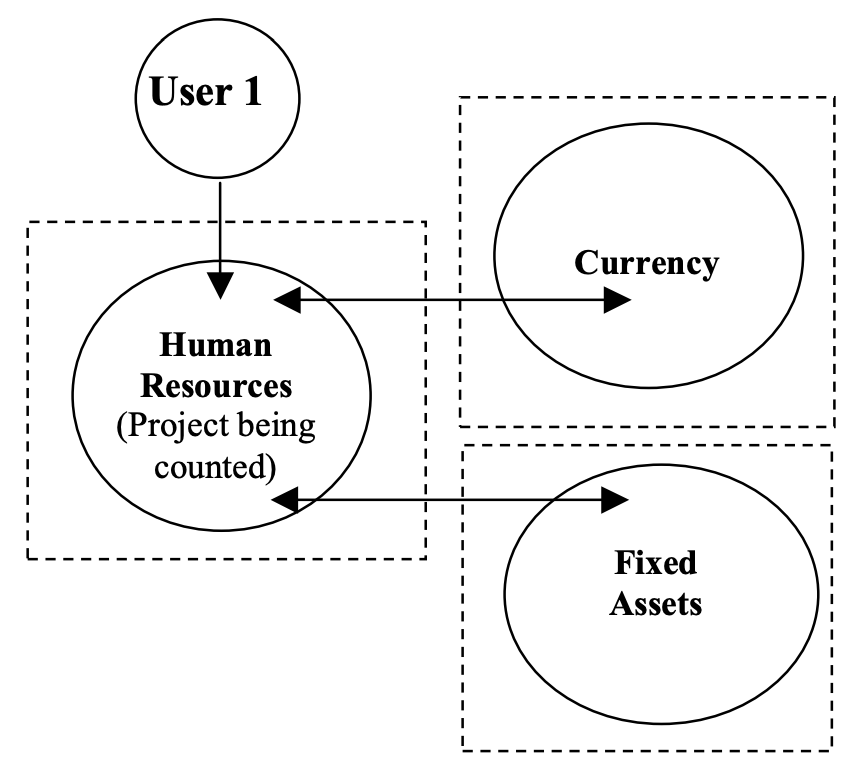
\includegraphics[width=\linewidth]{boundary.png}
\par\columnbreak\par
``The application \ul{boundary} indicates the border between the \ul{software} being measured and the \ul{user}.''\par
{\scriptsize Source: \bibentry{iso20926}\par}
\end{multicols}}

\pitch{\begin{multicols}{2}
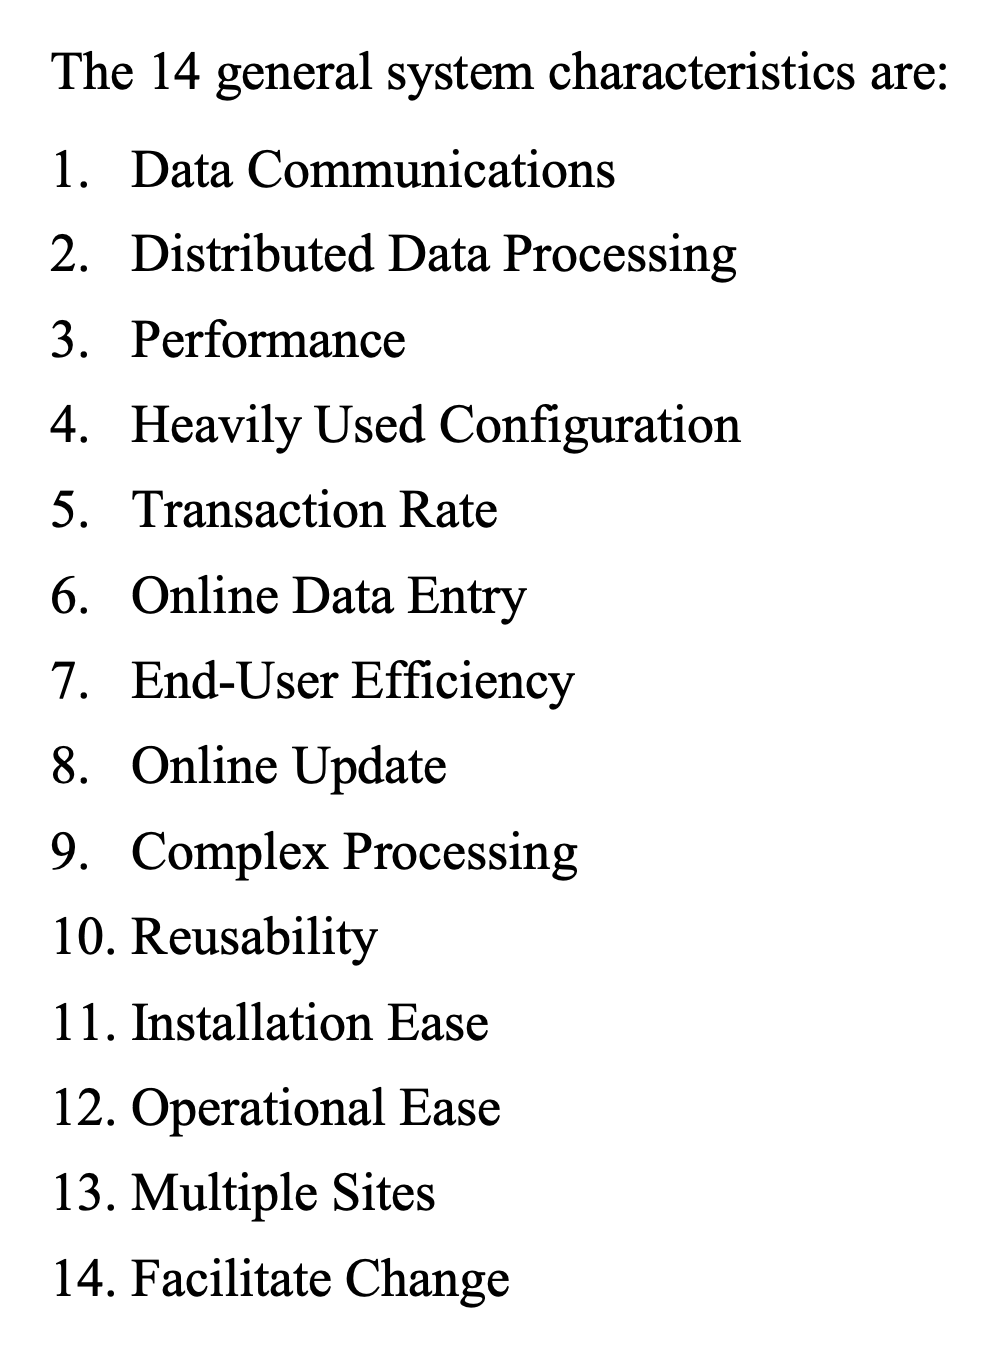
\includegraphics[width=.7\linewidth]{characteristics.png}
\par\columnbreak\par
``The 14 general system \ul{characteristics} are summarized into the \ul{value adjustment factor} (VAF). When applied, the value adjustment factor adjusts the \ul{unadjusted function point count} \(\pm\)35 percent to produce the \ul{adjusted function point count}.''\par
{\scriptsize Source: \bibentry{iso20926}\par}
\end{multicols}}

\pitch{\begin{multicols}{2}
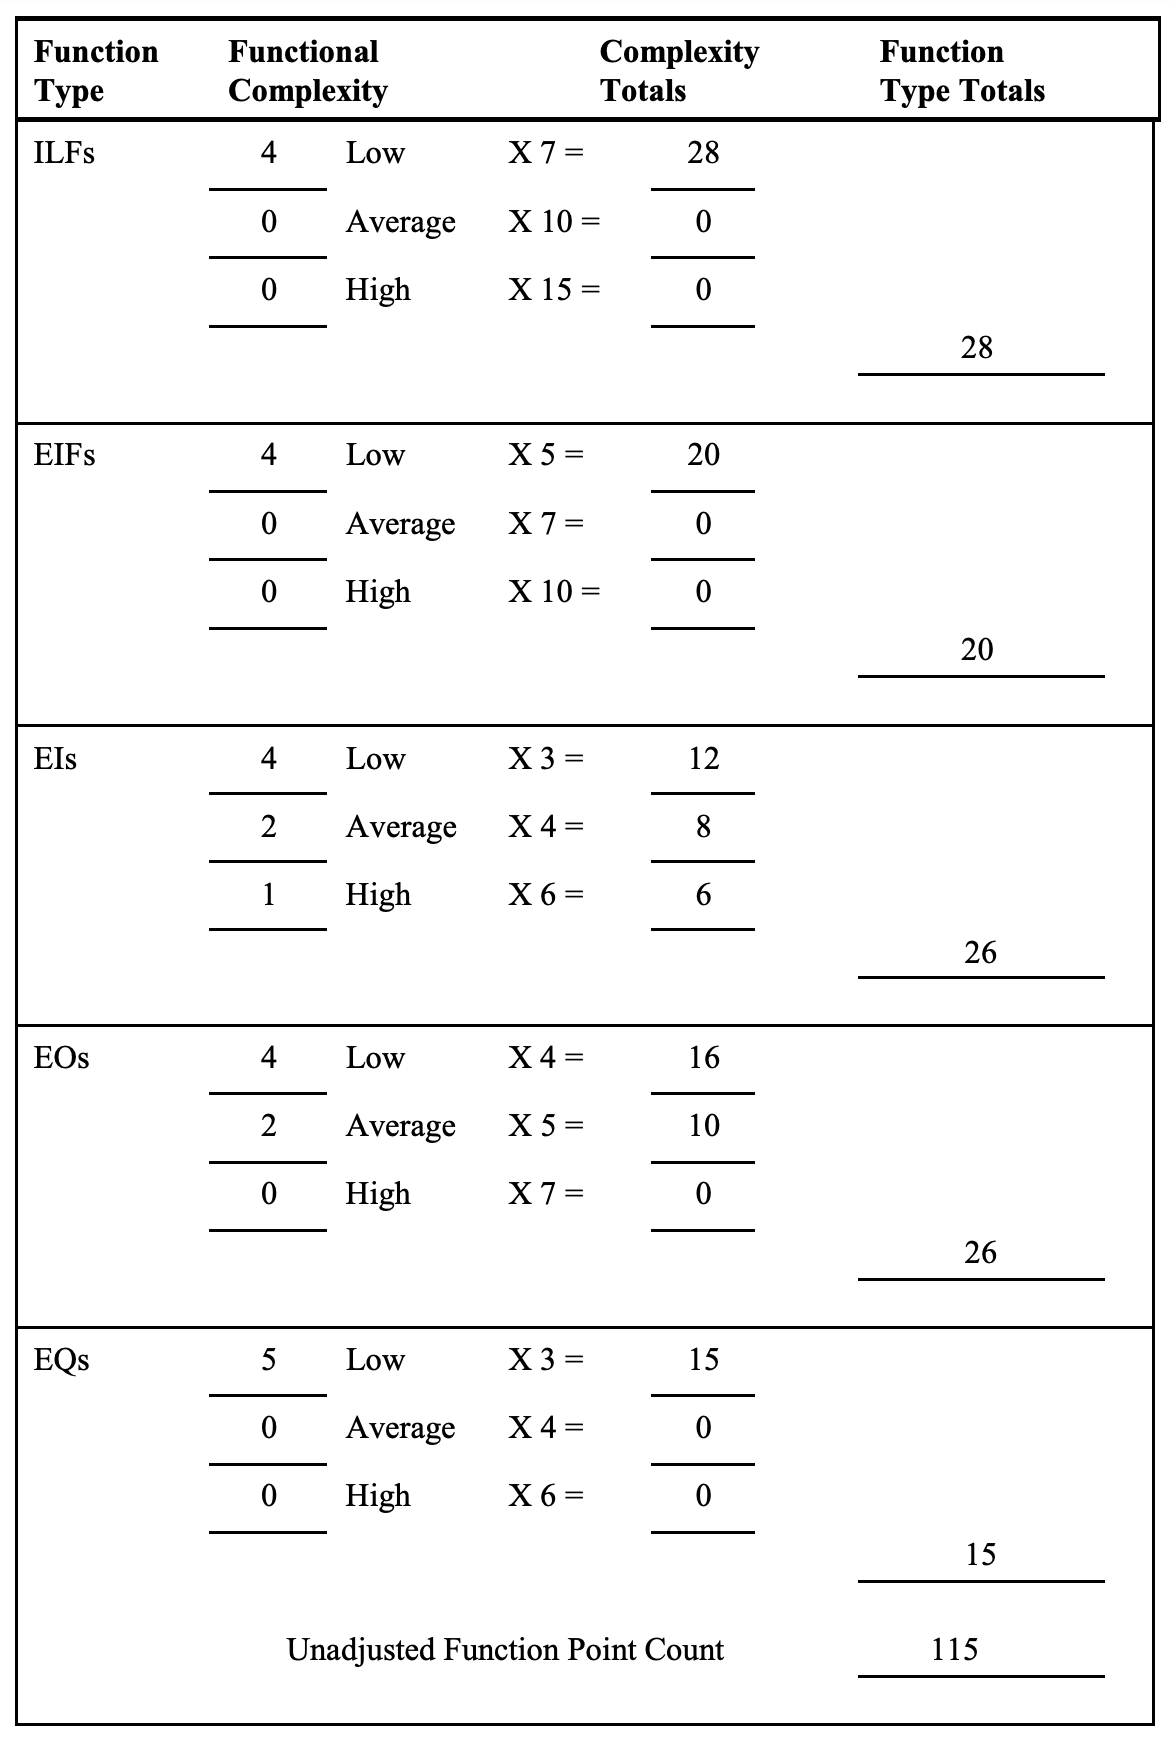
\includegraphics[width=.65\linewidth]{ufpc-example.png}
\par\columnbreak\par
``The formula calculates the \ul{development project function points}: \texttt{DFP = (UFP + CFP) * VAF}.
Where
UFP is the unadjusted function points for the functions that will be available after installation,
and
CFP is the unadjusted function points added by the conversion unadjusted function point count.''\par
{\scriptsize Source: \bibentry{iso20926}\par}
\end{multicols}}

\qte
  {book-of-charles-symons.jpg}
  {...}
  {symons1991software}

\pitch{\pptBanner{Function Points}
\begin{itemize}
\item Early and easy function points
\item COSMIC Function Points
\item Mk II Function Points
\item Nesma Function Points
\item FiSMA Function Points
\item Engineering function points
\item Object-Oriented Function Points (OOFP)
\item Weighted Micro Function Points
\item Fuzzy Function Points
\end{itemize}}

\pitch{Function Points may be measured by these tools:
\begin{itemize}
\item ...
\end{itemize}}

\end{document}
